% ============================================================
%  Trebuchet laser-cut parts -- cutting and assembly notes
%  4 kg oval build, 6 mm plywood, 900 x 600 bed
%  Compile: pdflatex (twice), beside the out/ folder
% ============================================================
\documentclass[11pt,a4paper]{article}
\usepackage[T1]{fontenc}
\usepackage[a4paper, top=1.2cm, bottom=1.6cm, left=1.5cm, right=1.5cm]{geometry}
\usepackage{xcolor}
\usepackage{graphicx}
\usepackage{tikz}
\usetikzlibrary{arrows.meta,calc,patterns}
\usepackage{booktabs}
\usepackage{array}
\usepackage{tabularx}
\usepackage{enumitem}
\usepackage{fancyhdr}
\usepackage[protrusion=true,expansion=false]{microtype}

\definecolor{Ink}{HTML}{1A1A1A}
\definecolor{HeadGrey}{HTML}{333333}
\definecolor{RuleGrey}{HTML}{888888}
\definecolor{BoxGrey}{HTML}{F0F0F0}
\definecolor{LineGrey}{HTML}{555555}
\definecolor{WarnBg}{HTML}{F5F5F5}
\definecolor{Wood}{HTML}{E2CFA8}
\definecolor{WoodDark}{HTML}{B8996A}
\definecolor{Steel}{HTML}{6B7178}
\definecolor{Alu}{HTML}{C9CED4}
\definecolor{Sand}{HTML}{D8C08A}
\definecolor{Strap}{HTML}{3E6C8C}
\definecolor{CutRed}{HTML}{FF0000}
\definecolor{EngBlue}{HTML}{0000FF}

\setlength{\parindent}{0pt}
\setlength{\parskip}{3pt}
\renewcommand{\arraystretch}{1.15}
\newcolumntype{L}[1]{>{\raggedright\arraybackslash}p{#1}}
\newcolumntype{Y}{>{\raggedright\arraybackslash}X}

\newcommand{\sechead}[1]{%
  \par\vspace{5pt}%
  {\bfseries\large\color{HeadGrey} #1}\\[-4pt]
  {\color{RuleGrey}\rule{\linewidth}{0.8pt}}\par\vspace{1pt}}
\newcommand{\warnbox}[1]{%
  \par\vspace{3pt}\noindent
  \fcolorbox{LineGrey}{WarnBg}{\parbox{\dimexpr\linewidth-2\fboxsep-2\fboxrule}{\small #1}}\par\vspace{3pt}}

\pagestyle{fancy}
\fancyhf{}
\renewcommand{\headrulewidth}{0pt}
\fancyfoot[L]{\footnotesize\color{RuleGrey} Trebuchet laser-cut parts \textbullet{} 4\,kg oval build \textbullet{} 6\,mm plywood}
\fancyfoot[R]{\footnotesize\color{RuleGrey} Page \thepage}

\tikzset{
  dim/.style={{Stealth[length=4pt]}-{Stealth[length=4pt]}, thin, Ink},
  ext/.style={very thin, RuleGrey},
  lbl/.style={font=\scriptsize, text=Ink, align=left},
  lead/.style={thin, LineGrey},
  dl/.style={font=\scriptsize, fill=white, inner sep=1pt, text=Ink},
}

\begin{document}
\small

{\LARGE\bfseries\color{Ink} Laser-cut parts --- 4\,kg oval trebuchet}\\[3pt]
{\color{RuleGrey}\rule{\linewidth}{1.2pt}}

These files cut the trebuchet's two A-frame sides and its small parts from \textbf{four sheets of 6\,mm plywood} on a \textbf{900 $\times$ 600\,mm} bed. Each side is two layers glued together (12\,mm). The arm stays a 40$\times$20$\times$1.6\,mm aluminium tube, and the base is timber: the laser can't cut either at this size. Sizes follow pages~8--9 of the Build Guide, changed for the 4\,kg limit: short arm 350, hang 280, and the axle 800 above the base rails.

\sechead{What is in the pack}
{\footnotesize
\begin{tabularx}{\linewidth}{@{}L{5.6cm} L{1.6cm} Y@{}}
\toprule
\textbf{File (.dxf and .svg)} & \textbf{Material} & \textbf{Parts} \\
\midrule
00\_Test\_coupon\_cut\_first & 6\,mm ply offcut & Fit test: axle and pin holes, tab slots \\
01\_Sheet\_SIDE\_A\_LAYER\_1 & 6\,mm ply & A-frame layer; trigger block (3 layers) and trigger base \\
02\_Sheet\_SIDE\_A\_LAYER\_2 & 6\,mm ply & A-frame layer; arm drilling templates (end and tip) \\
03\_Sheet\_SIDE\_B\_LAYER\_1 & 6\,mm ply & A-frame layer; two sensor plates \\
04\_Sheet\_SIDE\_B\_LAYER\_2 & 6\,mm ply & A-frame layer; marking templates for the aluminium doubler plates \\
05\_Fabric\_sling\_pouches & canvas or leather & Six sling pouches \\
gen.py & --- & The script that makes the files. Every size is a setting at the top. \\
\bottomrule
\end{tabularx}}

\textbf{Colours:} \textcolor{CutRed}{\textbf{red}} = cut through (layer CUT); \textcolor{EngBlue}{\textbf{blue}} = engrave or score lightly (layer ENGRAVE: labels and the screw marks for the brackets). Run the blue layer first, then the red; inside cuts before outlines. Everything is in millimetres at 1\,:\,1 --- check the import scale by measuring the 120\,mm boss on screen.

\sechead{Before you cut the big sheets}
\begin{enumerate}[itemsep=1pt, leftmargin=1.5em, topsep=1pt]
  \item \textbf{Cut the fit test} (00) from an offcut. The drawn hole sizes are nominal; your laser's kerf makes them a little bigger. Check which hole your 10\,mm trigger pin slides through freely, and that the three trigger layers (glued, 18\,mm) push into a tab slot snugly.
  \item \textbf{Check your bearings.} The side panels are drawn for a 20\,mm-bore \textbf{two-bolt flange bearing} with bolts \textbf{90\,mm apart} (the common UCFL204 pattern) and a 42\,mm clearance hole for its housing. Measure yours. If it differs, change \texttt{BEARING\_BOLT\_PITCH} and \texttt{BEARING\_CLEAR} in \texttt{gen.py} and run it again.
  \item If a fit is wrong, change the matching setting in \texttt{gen.py} (for example \texttt{PIN\_D}, \texttt{T} for thicker ply) and run \texttt{python3 gen.py}. It re-nests the sheets and checks that no parts overlap or leave the sheet.
\end{enumerate}

\sechead{Sheet layouts}
\begin{center}
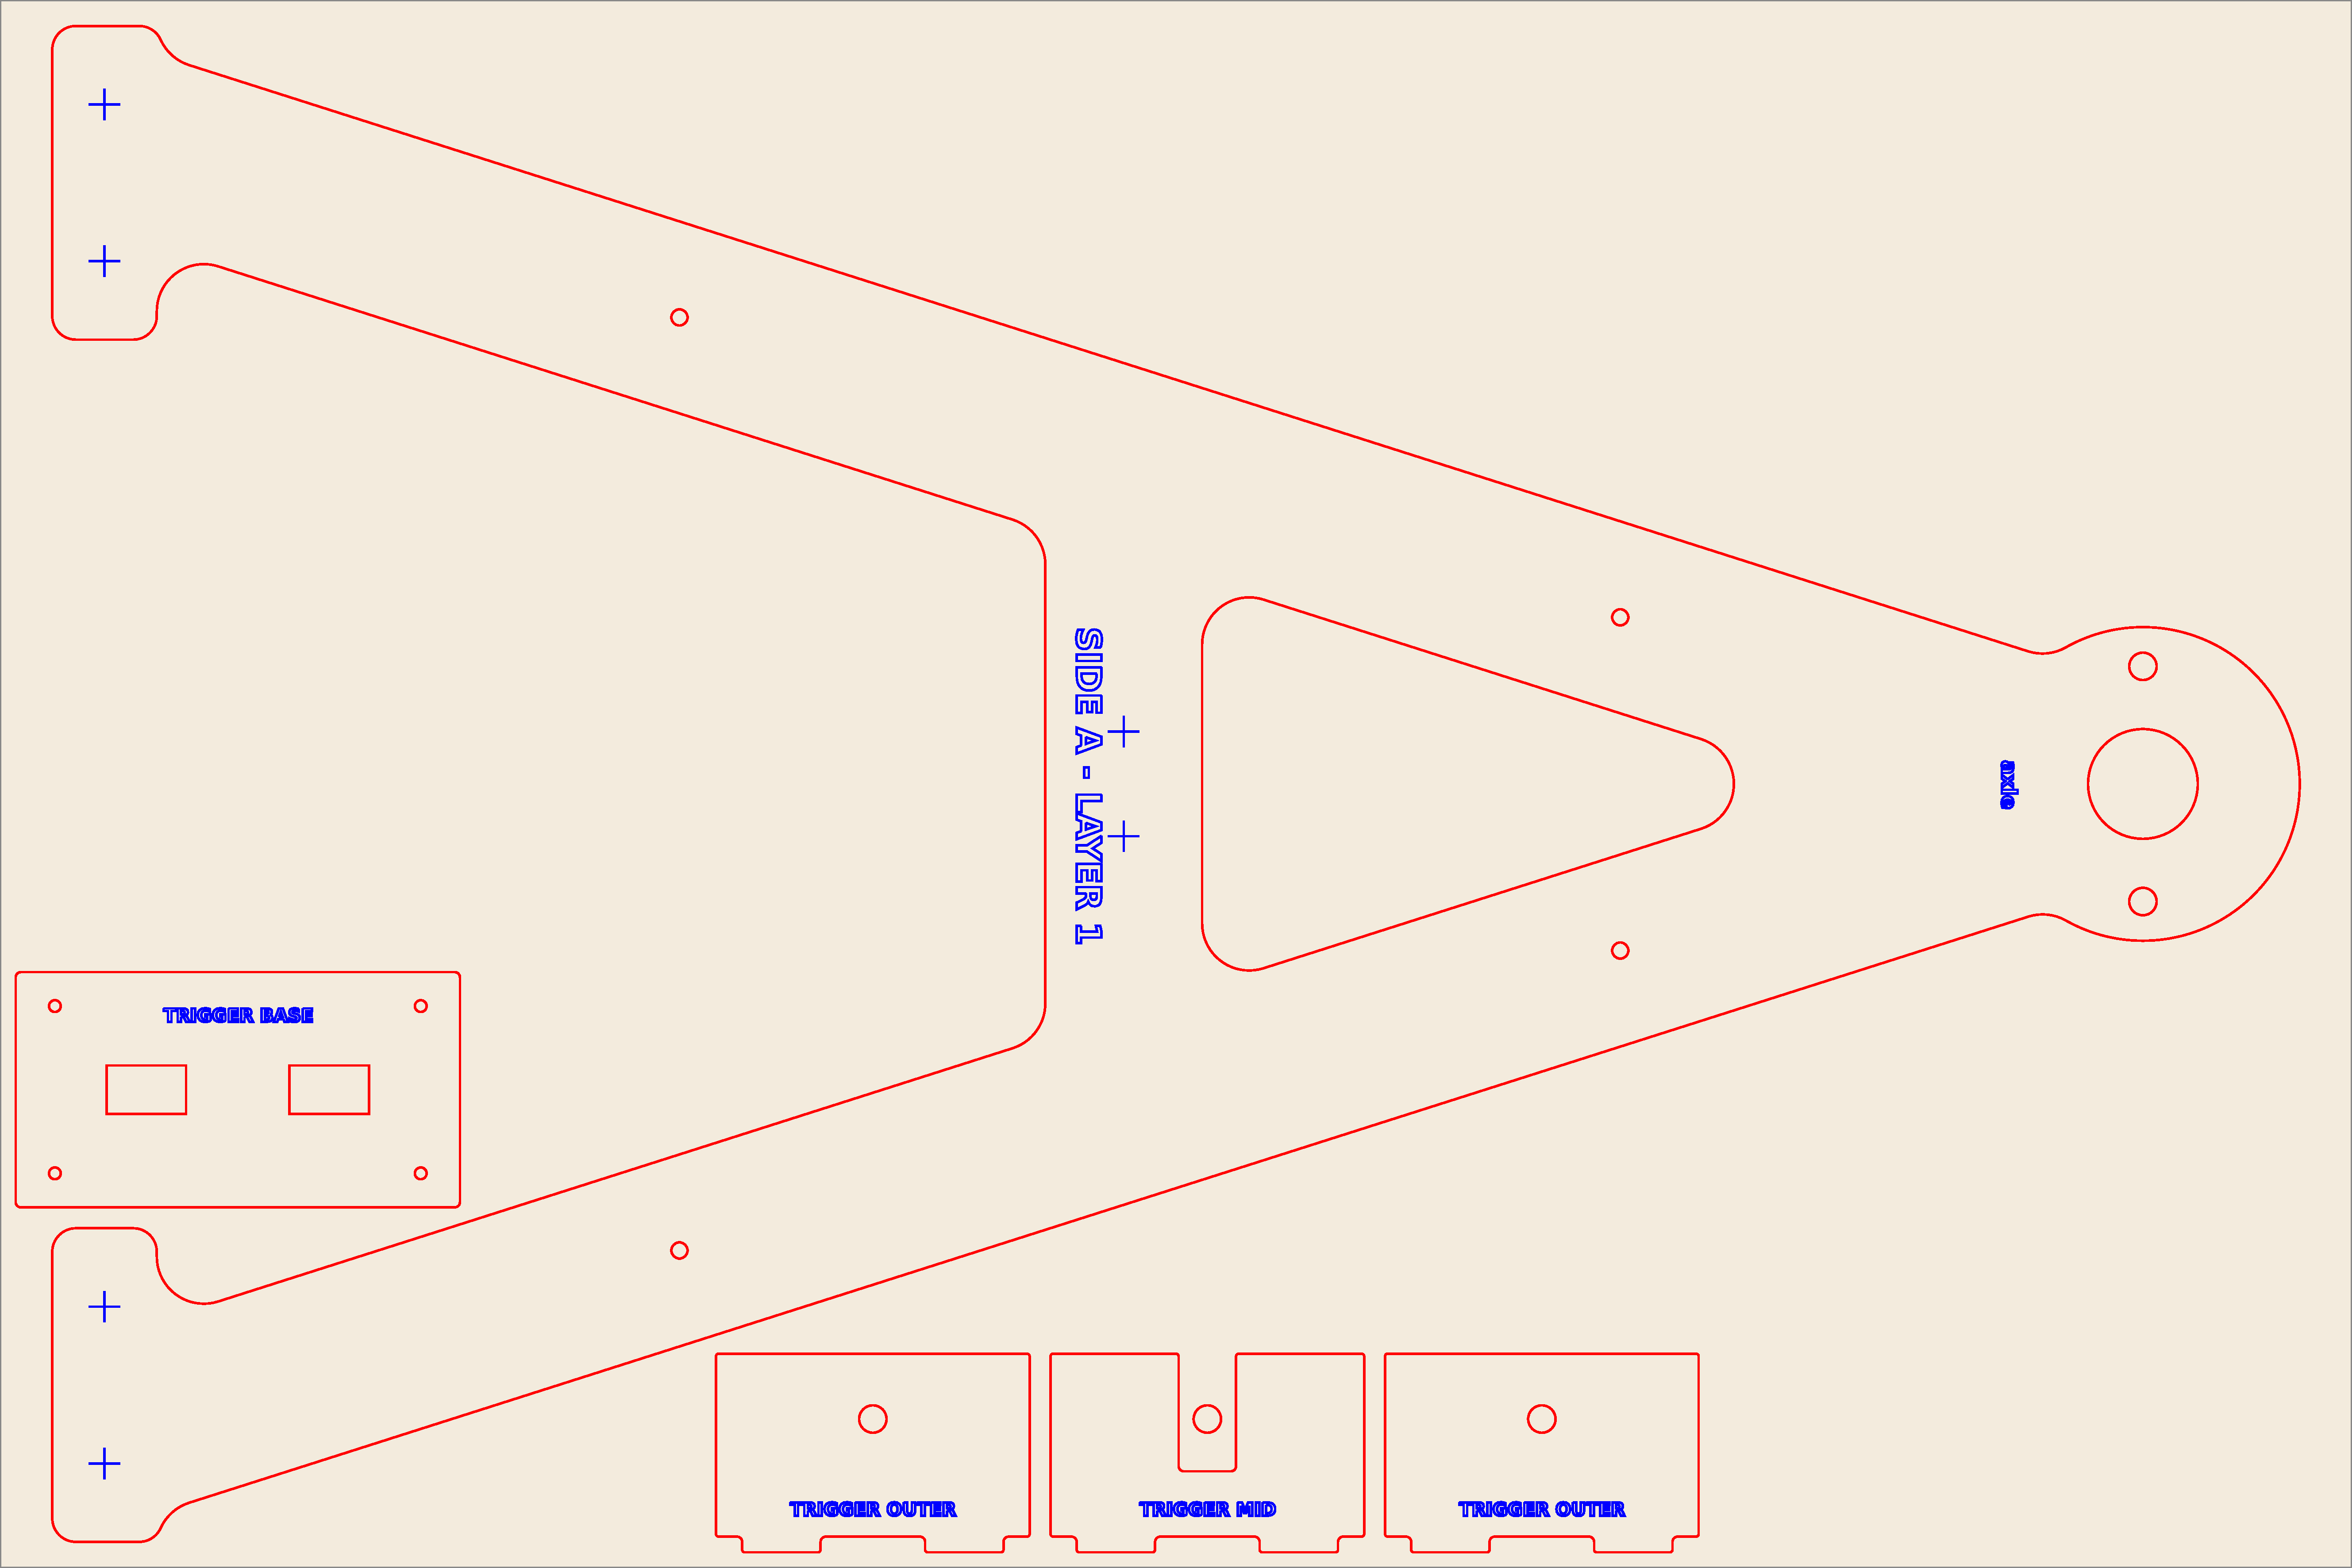
\includegraphics[width=0.43\linewidth]{out/01_Sheet_SIDE_A_LAYER_1_preview.pdf}\hspace{6mm}
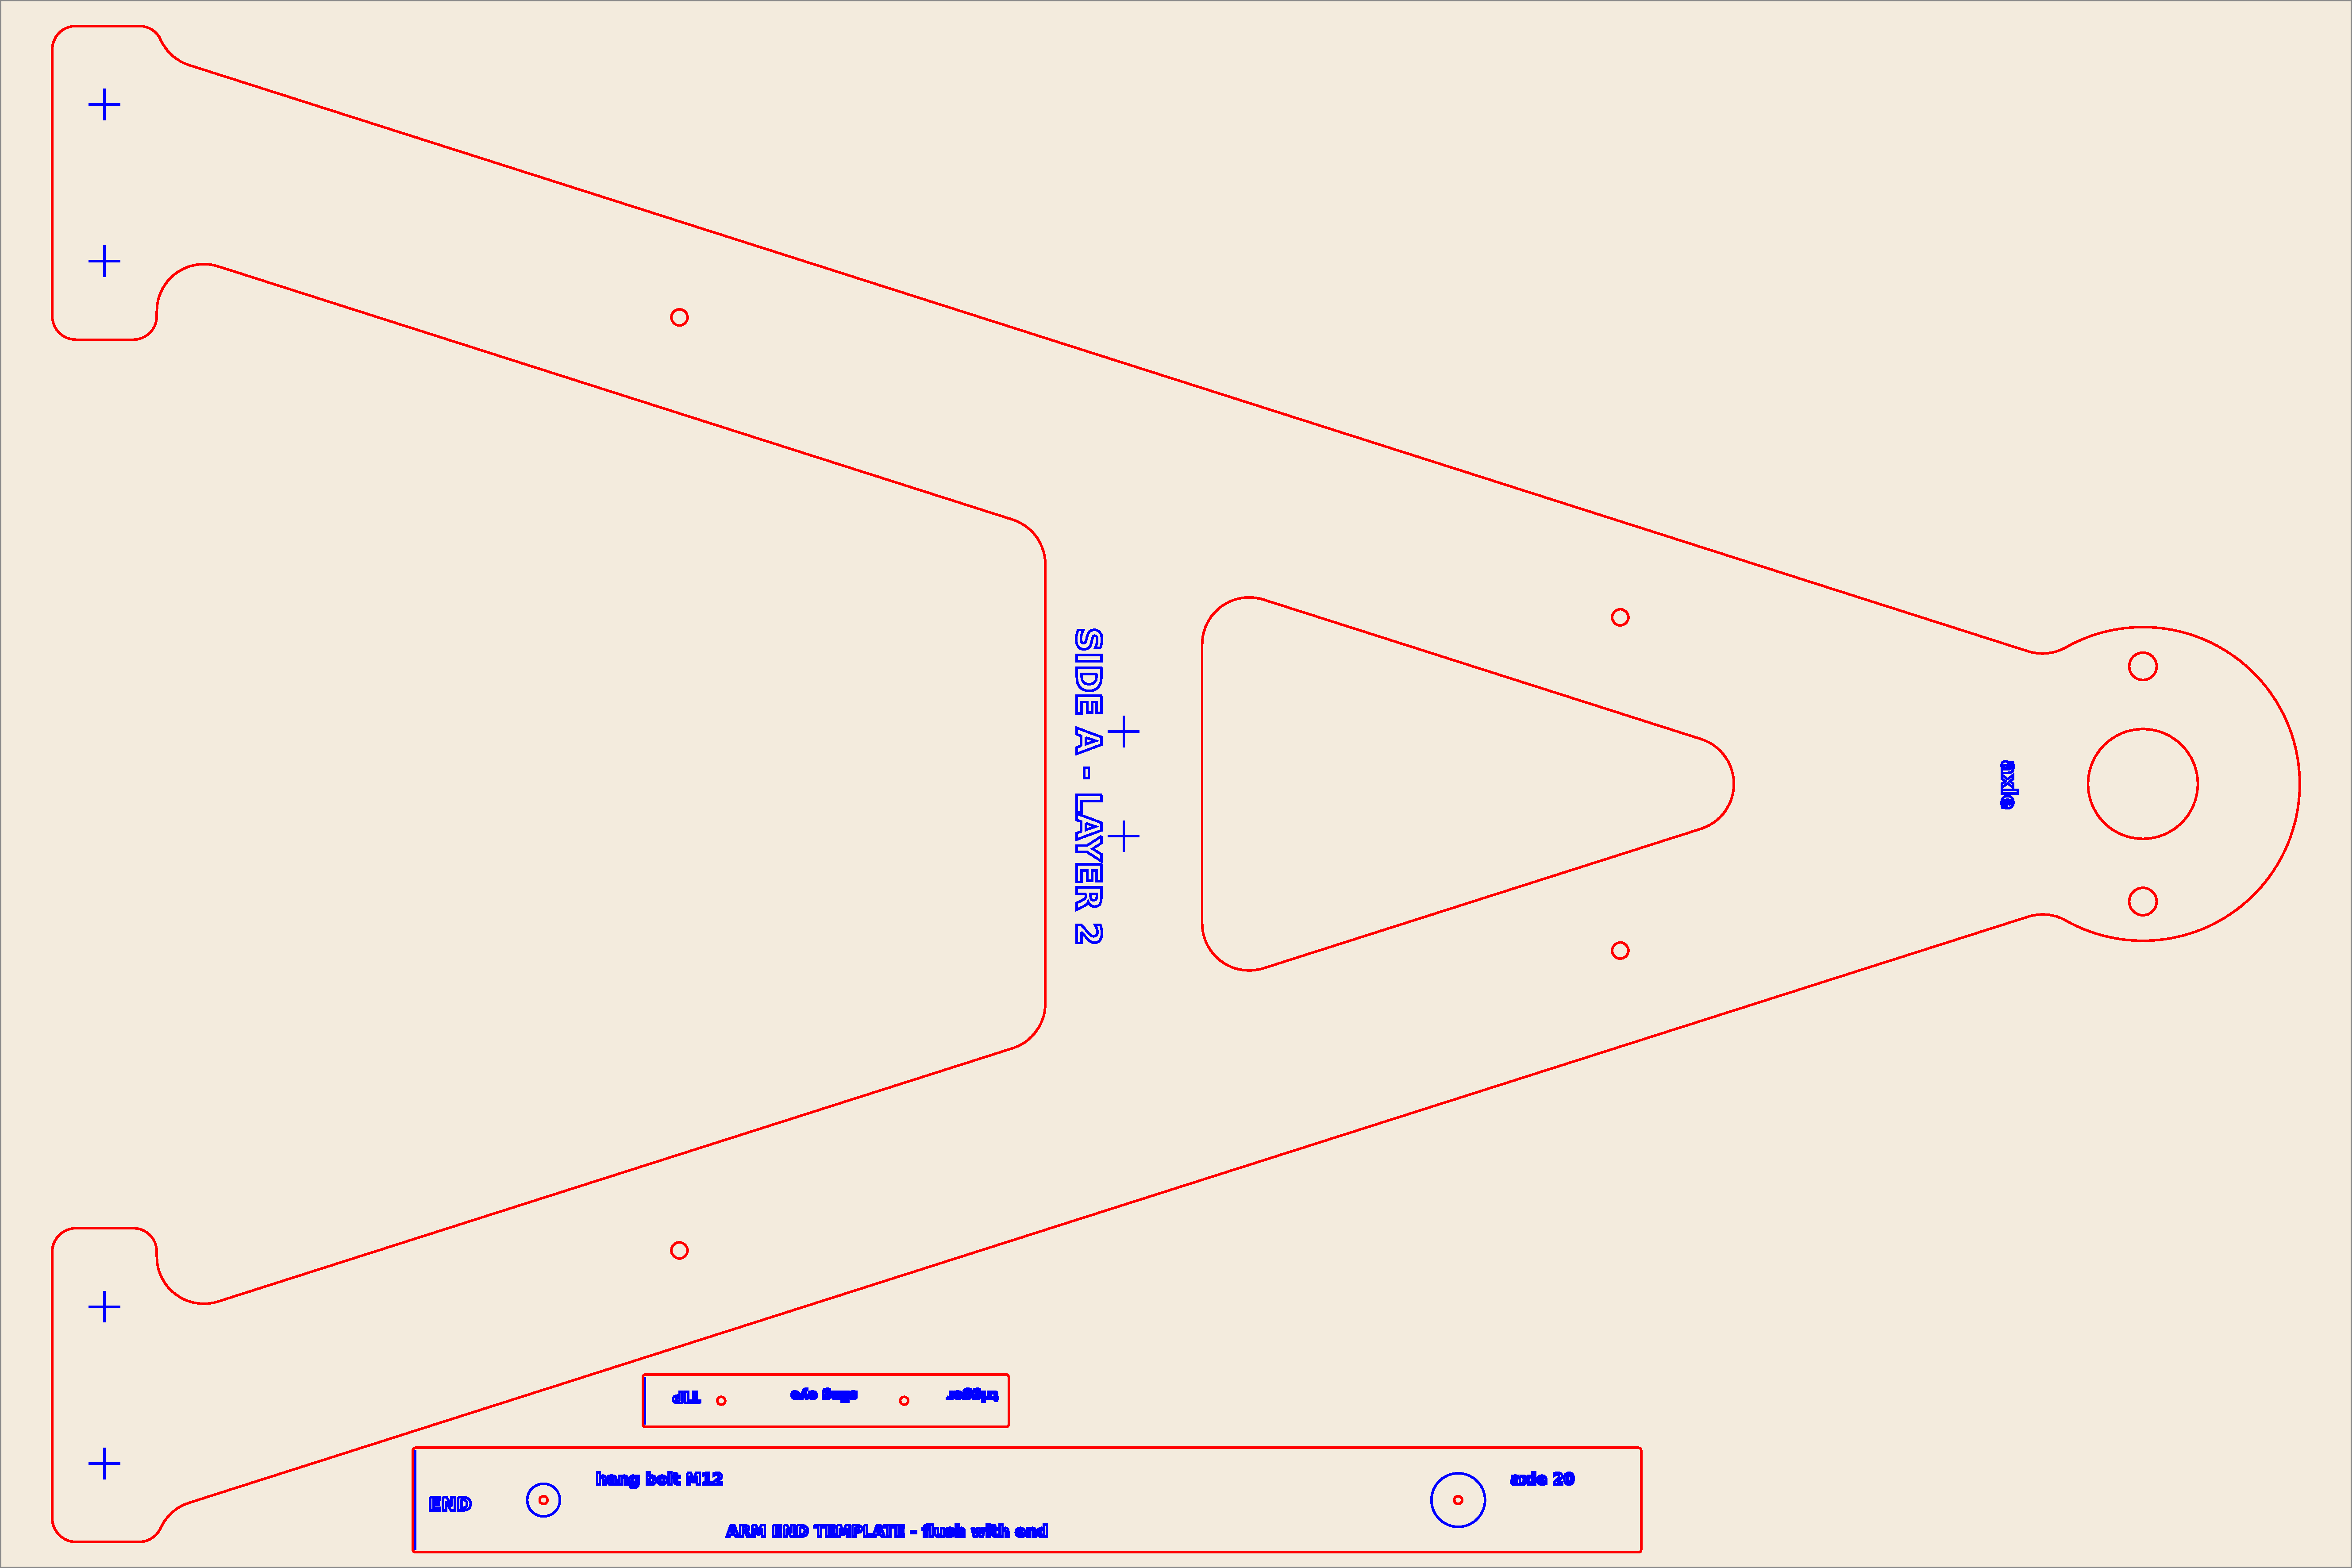
\includegraphics[width=0.43\linewidth]{out/02_Sheet_SIDE_A_LAYER_2_preview.pdf}\\[4pt]
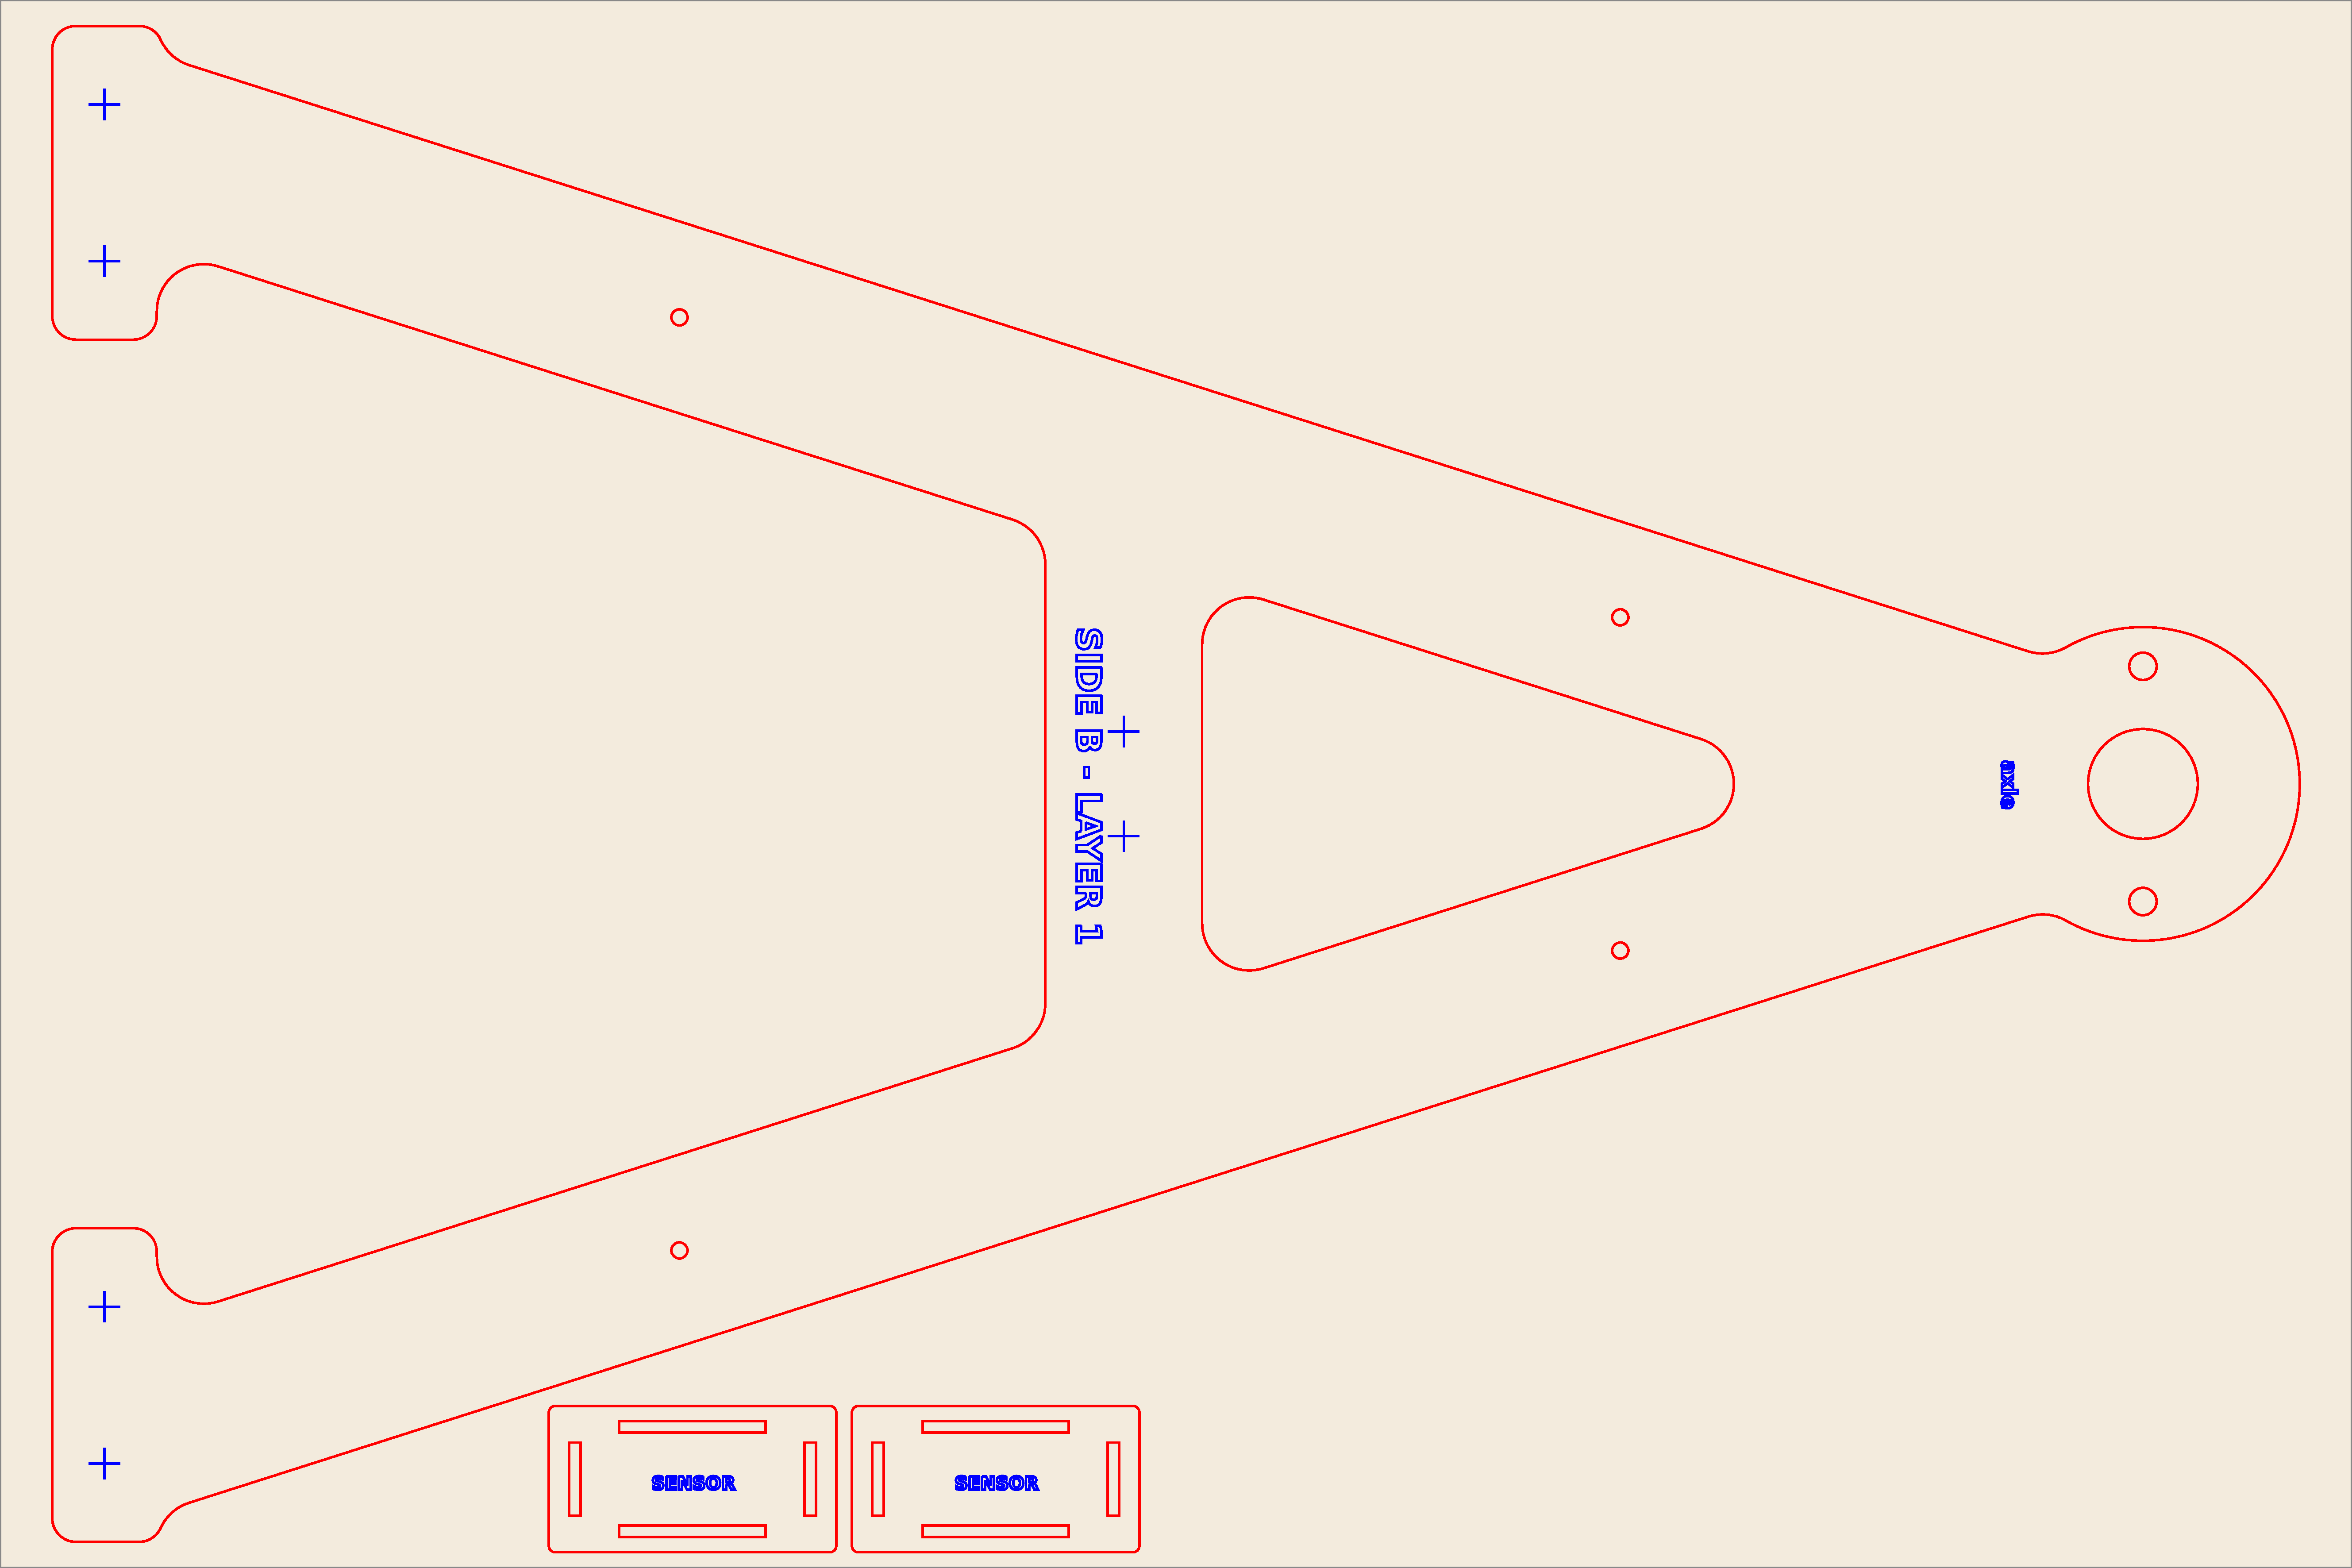
\includegraphics[width=0.43\linewidth]{out/03_Sheet_SIDE_B_LAYER_1_preview.pdf}\hspace{6mm}
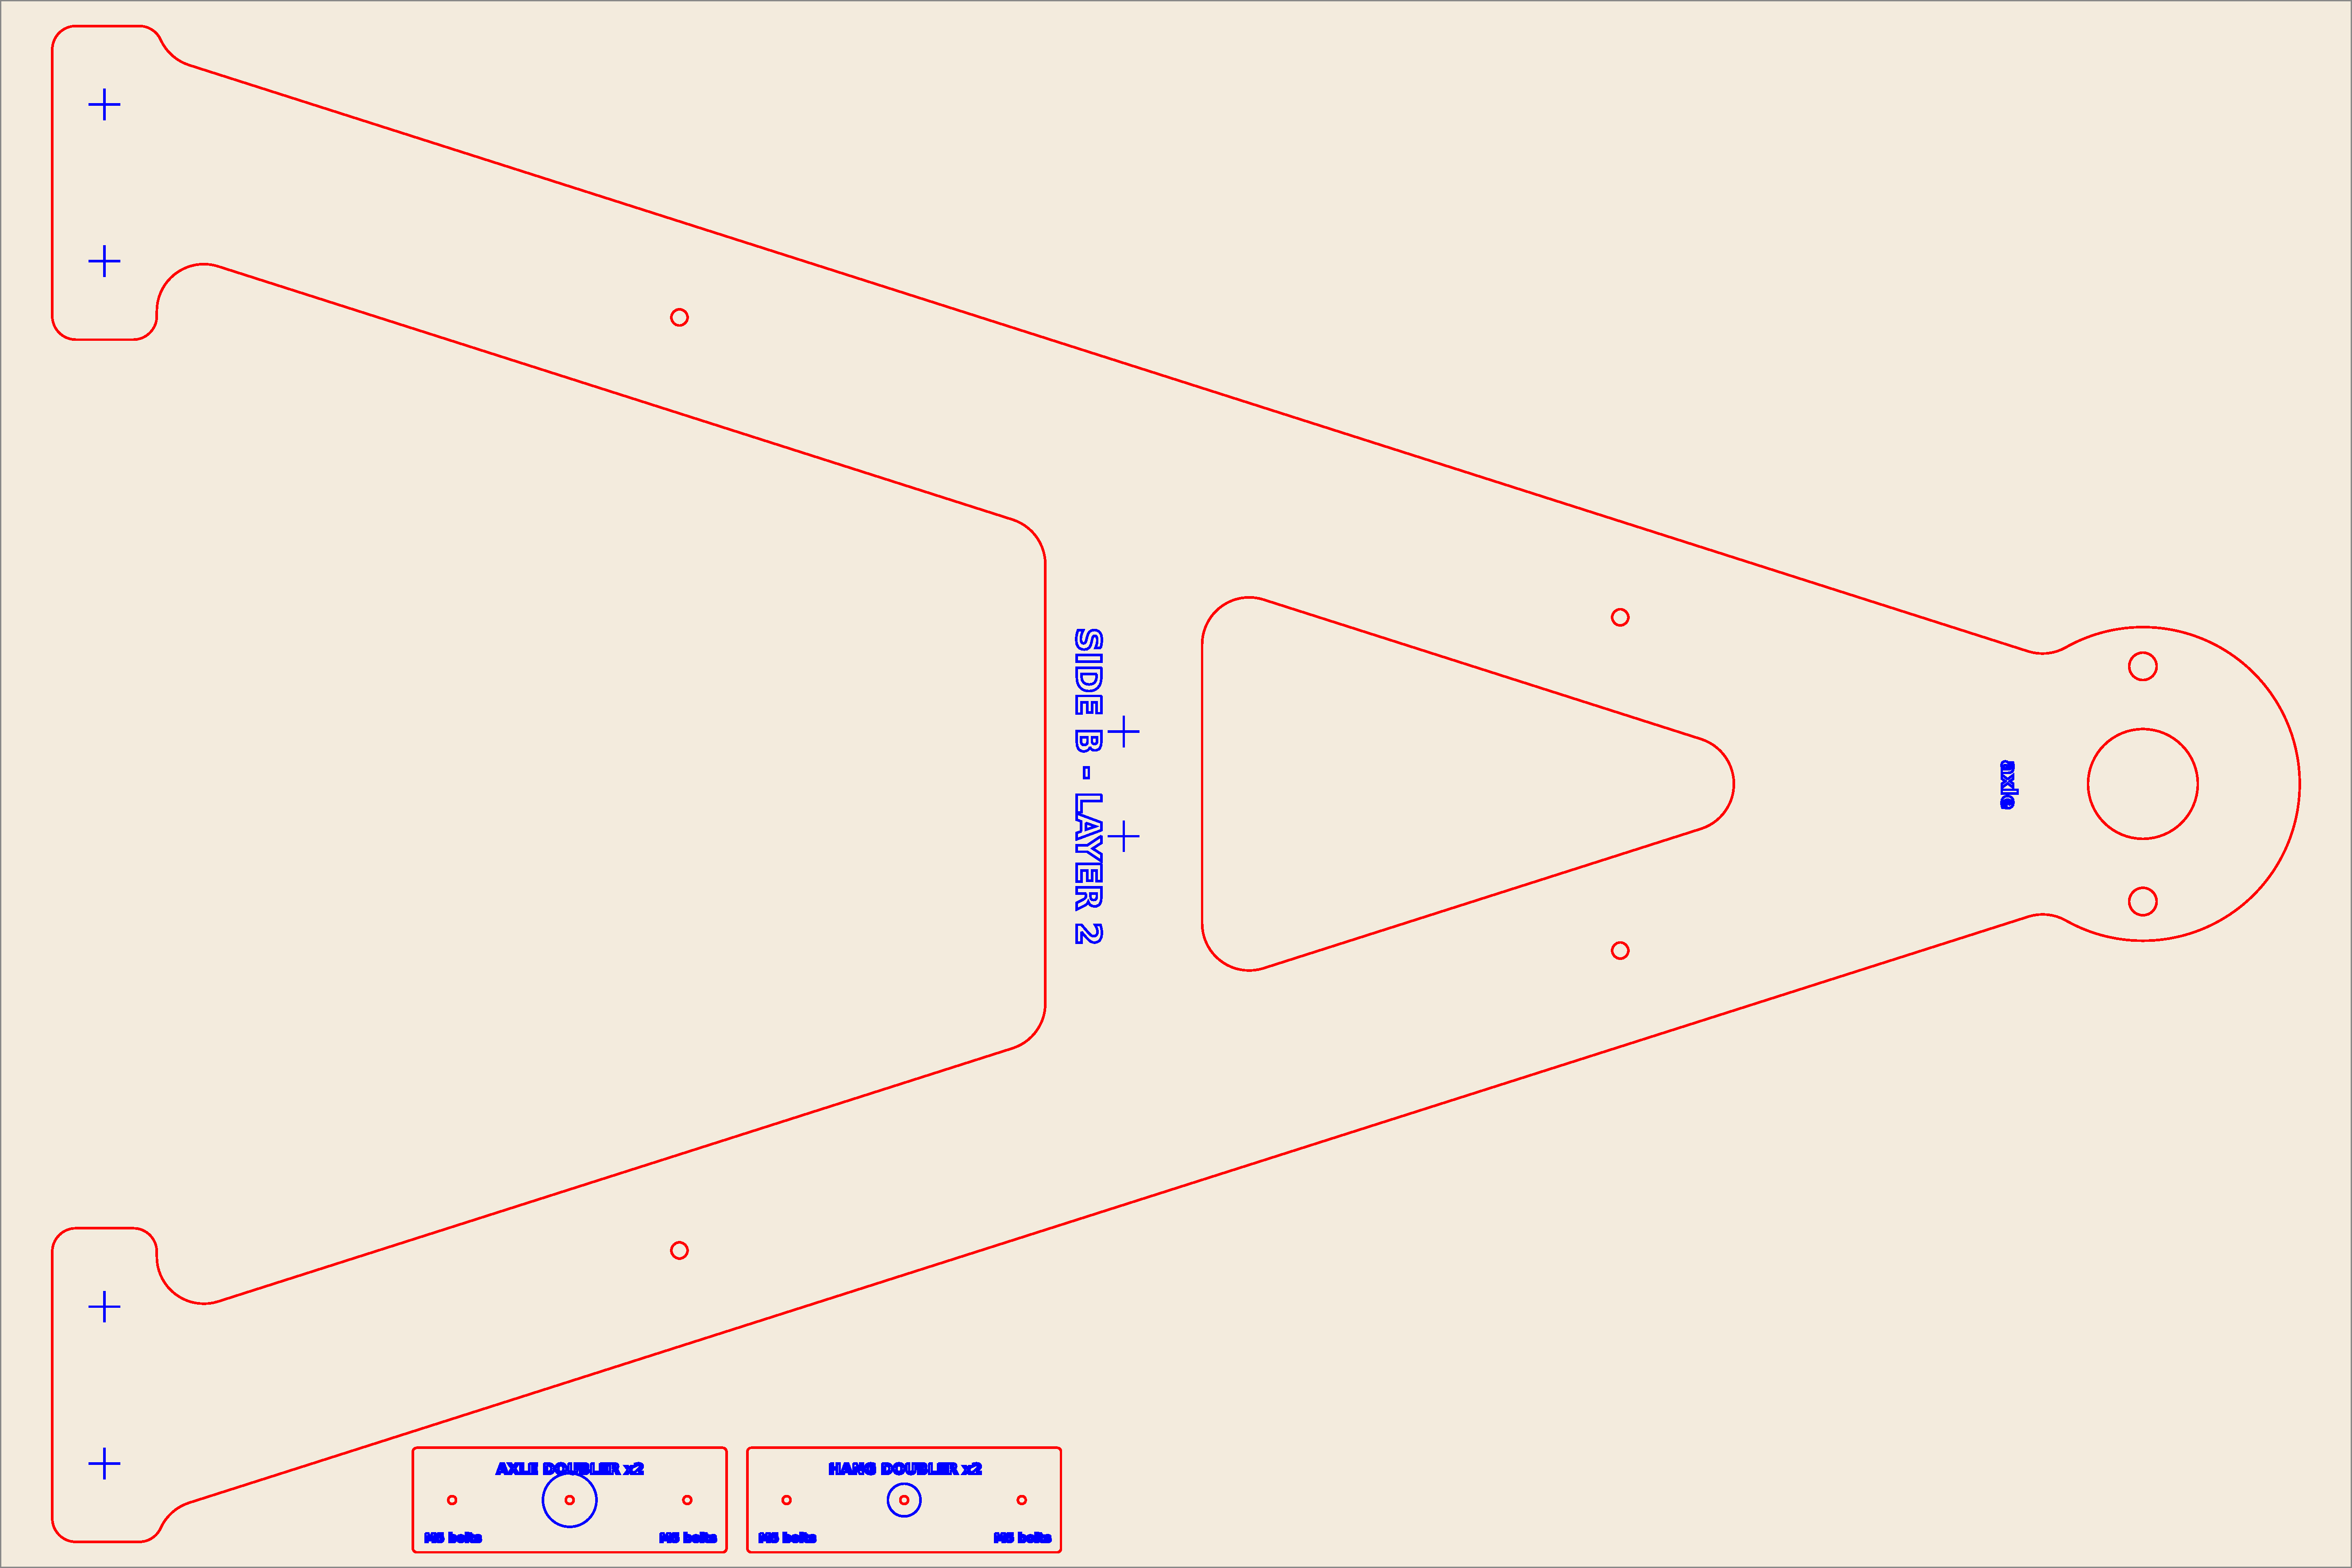
\includegraphics[width=0.43\linewidth]{out/04_Sheet_SIDE_B_LAYER_2_preview.pdf}
\end{center}

\newpage
\sechead{How it goes together}
\begin{center}
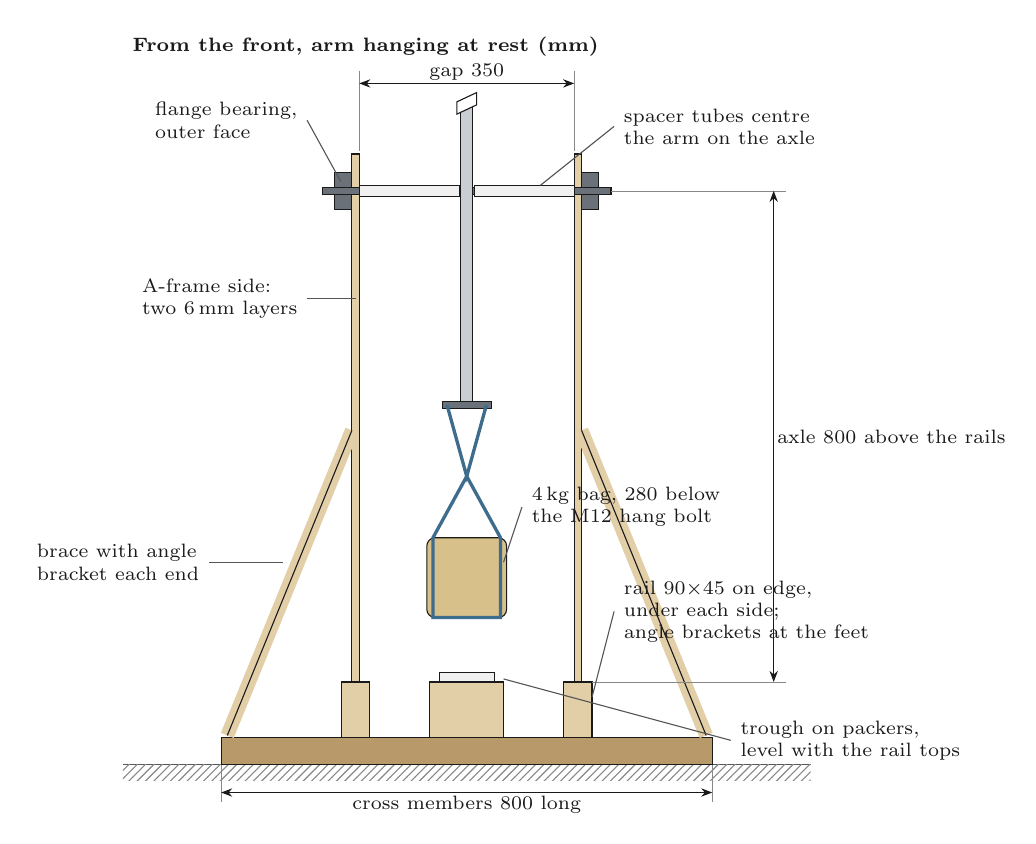
\begin{tikzpicture}[x=0.0078cm, y=0.0078cm]
  % ground
  \draw[LineGrey] (-560,0) -- (560,0);
  \fill[pattern=north east lines, pattern color=RuleGrey] (-560,-25) rectangle (560,0);
  % middle cross member (under the rails), outriggers to +-400
  \fill[WoodDark, draw=Ink, thin] (-400,0) rectangle (400,45);
  % rails on edge under the panels
  \fill[Wood, draw=Ink, thin] (-204,45) rectangle (-158,135);
  \fill[Wood, draw=Ink, thin] (158,45) rectangle (204,135);
  % panels (edge-on, 12 thick) from rail top to boss top
  \fill[Wood, draw=Ink, thin] (-187,135) rectangle (-175,995);
  \fill[Wood, draw=Ink, thin] (175,135) rectangle (187,995);
  % bearings on outer faces
  \fill[Steel, draw=Ink, thin] (-215,905) rectangle (-187,965);
  \fill[Steel, draw=Ink, thin] (187,905) rectangle (215,965);
  % axle
  \fill[Steel, draw=Ink, thin] (-235,929) rectangle (235,941);
  % spacers
  \fill[BoxGrey, draw=Ink, thin] (-175,926) rectangle (-12,944);
  \fill[BoxGrey, draw=Ink, thin] (12,926) rectangle (175,944);
  % arm end-on at rest (hanging) -- 20 wide
  \fill[Alu, draw=Ink, thin] (-10,585) rectangle (10,1080);
  \draw[Ink, thin, fill=white] (-16,1060) -- (16,1075) -- (16,1095) -- (-16,1080) -- cycle;
  % hang bolt at 350 below axle, bag 280 below that
  \fill[Steel, draw=Ink, thin] (-40,580) rectangle (40,592);
  \draw[Strap, line width=1.2pt] (-32,586) -- (0,470) -- (32,586);
  \fill[Sand, draw=Ink, thin, rounded corners=3pt] (-65,240) rectangle (65,370);
  \draw[Strap, line width=1.2pt] (0,470) -- (-55,370) -- (-55,240) -- (55,240) -- (55,370) -- cycle;
  % braces
  \draw[Wood, line width=5pt] (-187,545) -- (-390,48);
  \draw[Wood, line width=5pt] (187,545) -- (390,48);
  \draw[Ink, thin] (-187,545) -- (-390,48); \draw[Ink, thin] (187,545) -- (390,48);
  % trough on packers
  \fill[BoxGrey, draw=Ink, thin] (-45,135) rectangle (45,150);
  \fill[Wood, draw=Ink, thin] (-60,45) rectangle (60,135);
  % dims
  \draw[ext] (-175,1000) -- (-175,1130); \draw[ext] (175,1000) -- (175,1130);
  \draw[dim] (-175,1110) -- (175,1110) node[midway, above, dl] {gap 350};
  \draw[ext] (235,935) -- (520,935); \draw[ext] (204,135) -- (520,135);
  \draw[dim] (500,135) -- (500,935) node[midway, right, dl] {axle 800 above the rails};
  \draw[ext] (-400,0) -- (-400,-60); \draw[ext] (400,0) -- (400,-60);
  \draw[dim] (-400,-45) -- (400,-45) node[midway, below, dl] {cross members 800 long};
  % labels
  \node[lbl, anchor=east] (a) at (-260,1050) {flange bearing,\\outer face};
  \draw[lead] (a.east) -- (-205,950);
  \node[lbl, anchor=east] (b) at (-260,760) {A-frame side:\\two 6\,mm layers};
  \draw[lead] (b.east) -- (-181,760);
  \node[lbl, anchor=east] (c) at (-420,330) {brace with angle\\bracket each end};
  \draw[lead] (c.east) -- (-300,330);
  \node[lbl, anchor=west] (d) at (240,250) {rail 90$\times$45 on edge,\\under each side;\\angle brackets at the feet};
  \draw[lead] (d.west) -- (204,110);
  \node[lbl, anchor=west] (e) at (90,420) {4\,kg bag, 280 below\\the M12 hang bolt};
  \draw[lead] (e.west) -- (60,330);
  \node[lbl, anchor=west] (f) at (240,1040) {spacer tubes centre\\the arm on the axle};
  \draw[lead] (f.west) -- (120,944);
  \node[lbl, anchor=west] (g) at (430,40) {trough on packers,\\level with the rail tops};
  \draw[lead] (g.west) -- (60,140);
  \node[lbl, anchor=west] at (-560,1170) {\bfseries From the front, arm hanging at rest (mm)};
\end{tikzpicture}
\end{center}

\begin{minipage}[t]{0.49\linewidth}
\sechead{Assembly}
\begin{enumerate}[itemsep=1pt, leftmargin=1.5em, topsep=1pt]
  \item \textbf{Glue each pair} of A-frame layers (A1+A2, B1+B2) with PVA. Push 6\,mm dowels through the five dowel holes to line them up; engraved faces outward. Clamp flat on a bench overnight; trim the dowels flush.
  \item \textbf{Base:} lay the three cross members (front, back, and one under the pivot line), then screw the two rails across them, on edge, 362\,mm apart centre to centre, so they sit under the panels.
  \item \textbf{Stand the sides} on the rails, feet over the rails, inside faces 350\,mm apart. Fix each foot with two angle brackets at the engraved crosses.
  \item \textbf{Braces:} from the engraved crosses on each crossbar down to the ends of the middle cross member, with an angle bracket each end.
  \item \textbf{Bearings} on the outer faces. Drill the arm with the templates (axle 400 from the end, hang bolt 50 from the end), bolt on the doubler plates, then thread the axle: bearing, spacer, arm, spacer, bearing. Collars outside the bearings.
  \item \textbf{Trigger:} glue the three trigger layers (slotted one in the middle), push the tabs into the trigger base, and screw the base to the back cross member under the cocked arm's trigger eye.
  \item \textbf{Sensor plate:} strap to the arm 100--150\,mm from the axle; strap the sensor to the plate.
  \item Sling, pouch, beanbags and safety: Build Guide pages 5--9.
\end{enumerate}
\end{minipage}\hfill
\begin{minipage}[t]{0.48\linewidth}
\sechead{Also needed}
{\footnotesize
\begin{tabularx}{\linewidth}{@{}Y L{1.2cm}@{}}
\toprule
\textbf{Item} & \textbf{Qty} \\
\midrule
6\,mm plywood, 900$\times$600 & 4 sheets \\
Aluminium tube 40$\times$20$\times$1.6, 1400 long & 1 \\
6\,mm aluminium plate, 120$\times$40 (doublers) & 4 \\
2-bolt flange bearing, 20\,mm bore + M10 bolts & 2 + 4 \\
20\,mm steel axle, 420 long; 2 shaft collars & 1 \\
Spacer tube (25\,mm conduit), 163 long & 2 \\
M12$\times$50 hang bolt, nyloc nut, washers & 1 \\
M5$\times$40 bolts for doublers & 8 \\
M6 eye bolts (sling eye, trigger eye) & 2 \\
10\,mm trigger pin (rod or clevis pin) & 1 \\
Pine 90$\times$45: rails 1500; cross members 800 & 2; 3 \\
Pine 70$\times$35 braces, about 560 & 2 \\
Steel angle brackets 50\,mm & 8 \\
6\,mm dowel, 30 long & 10 \\
90\,mm PVC pipe, halved, 1200 long (trough) & 1 \\
Rated strap cradle and shackle (Guide p.\,9) & 1 \\
\bottomrule
\end{tabularx}}
\warnbox{\textbf{Before the first launch} check: the arm swings a full turn by hand without touching anything; the bag clears the base by at least 80\,mm at the bottom of its swing; the bearing bolts and the hang bolt are tight; and the frame is pegged or sandbagged. The aluminium doublers are \textbf{not} laser-cut --- use the templates on sheet~4 to mark and drill them.}
\end{minipage}


\end{document}
